\chapter{Psycholinguistik}
\begin{figure}[htbp]
\begin{center}
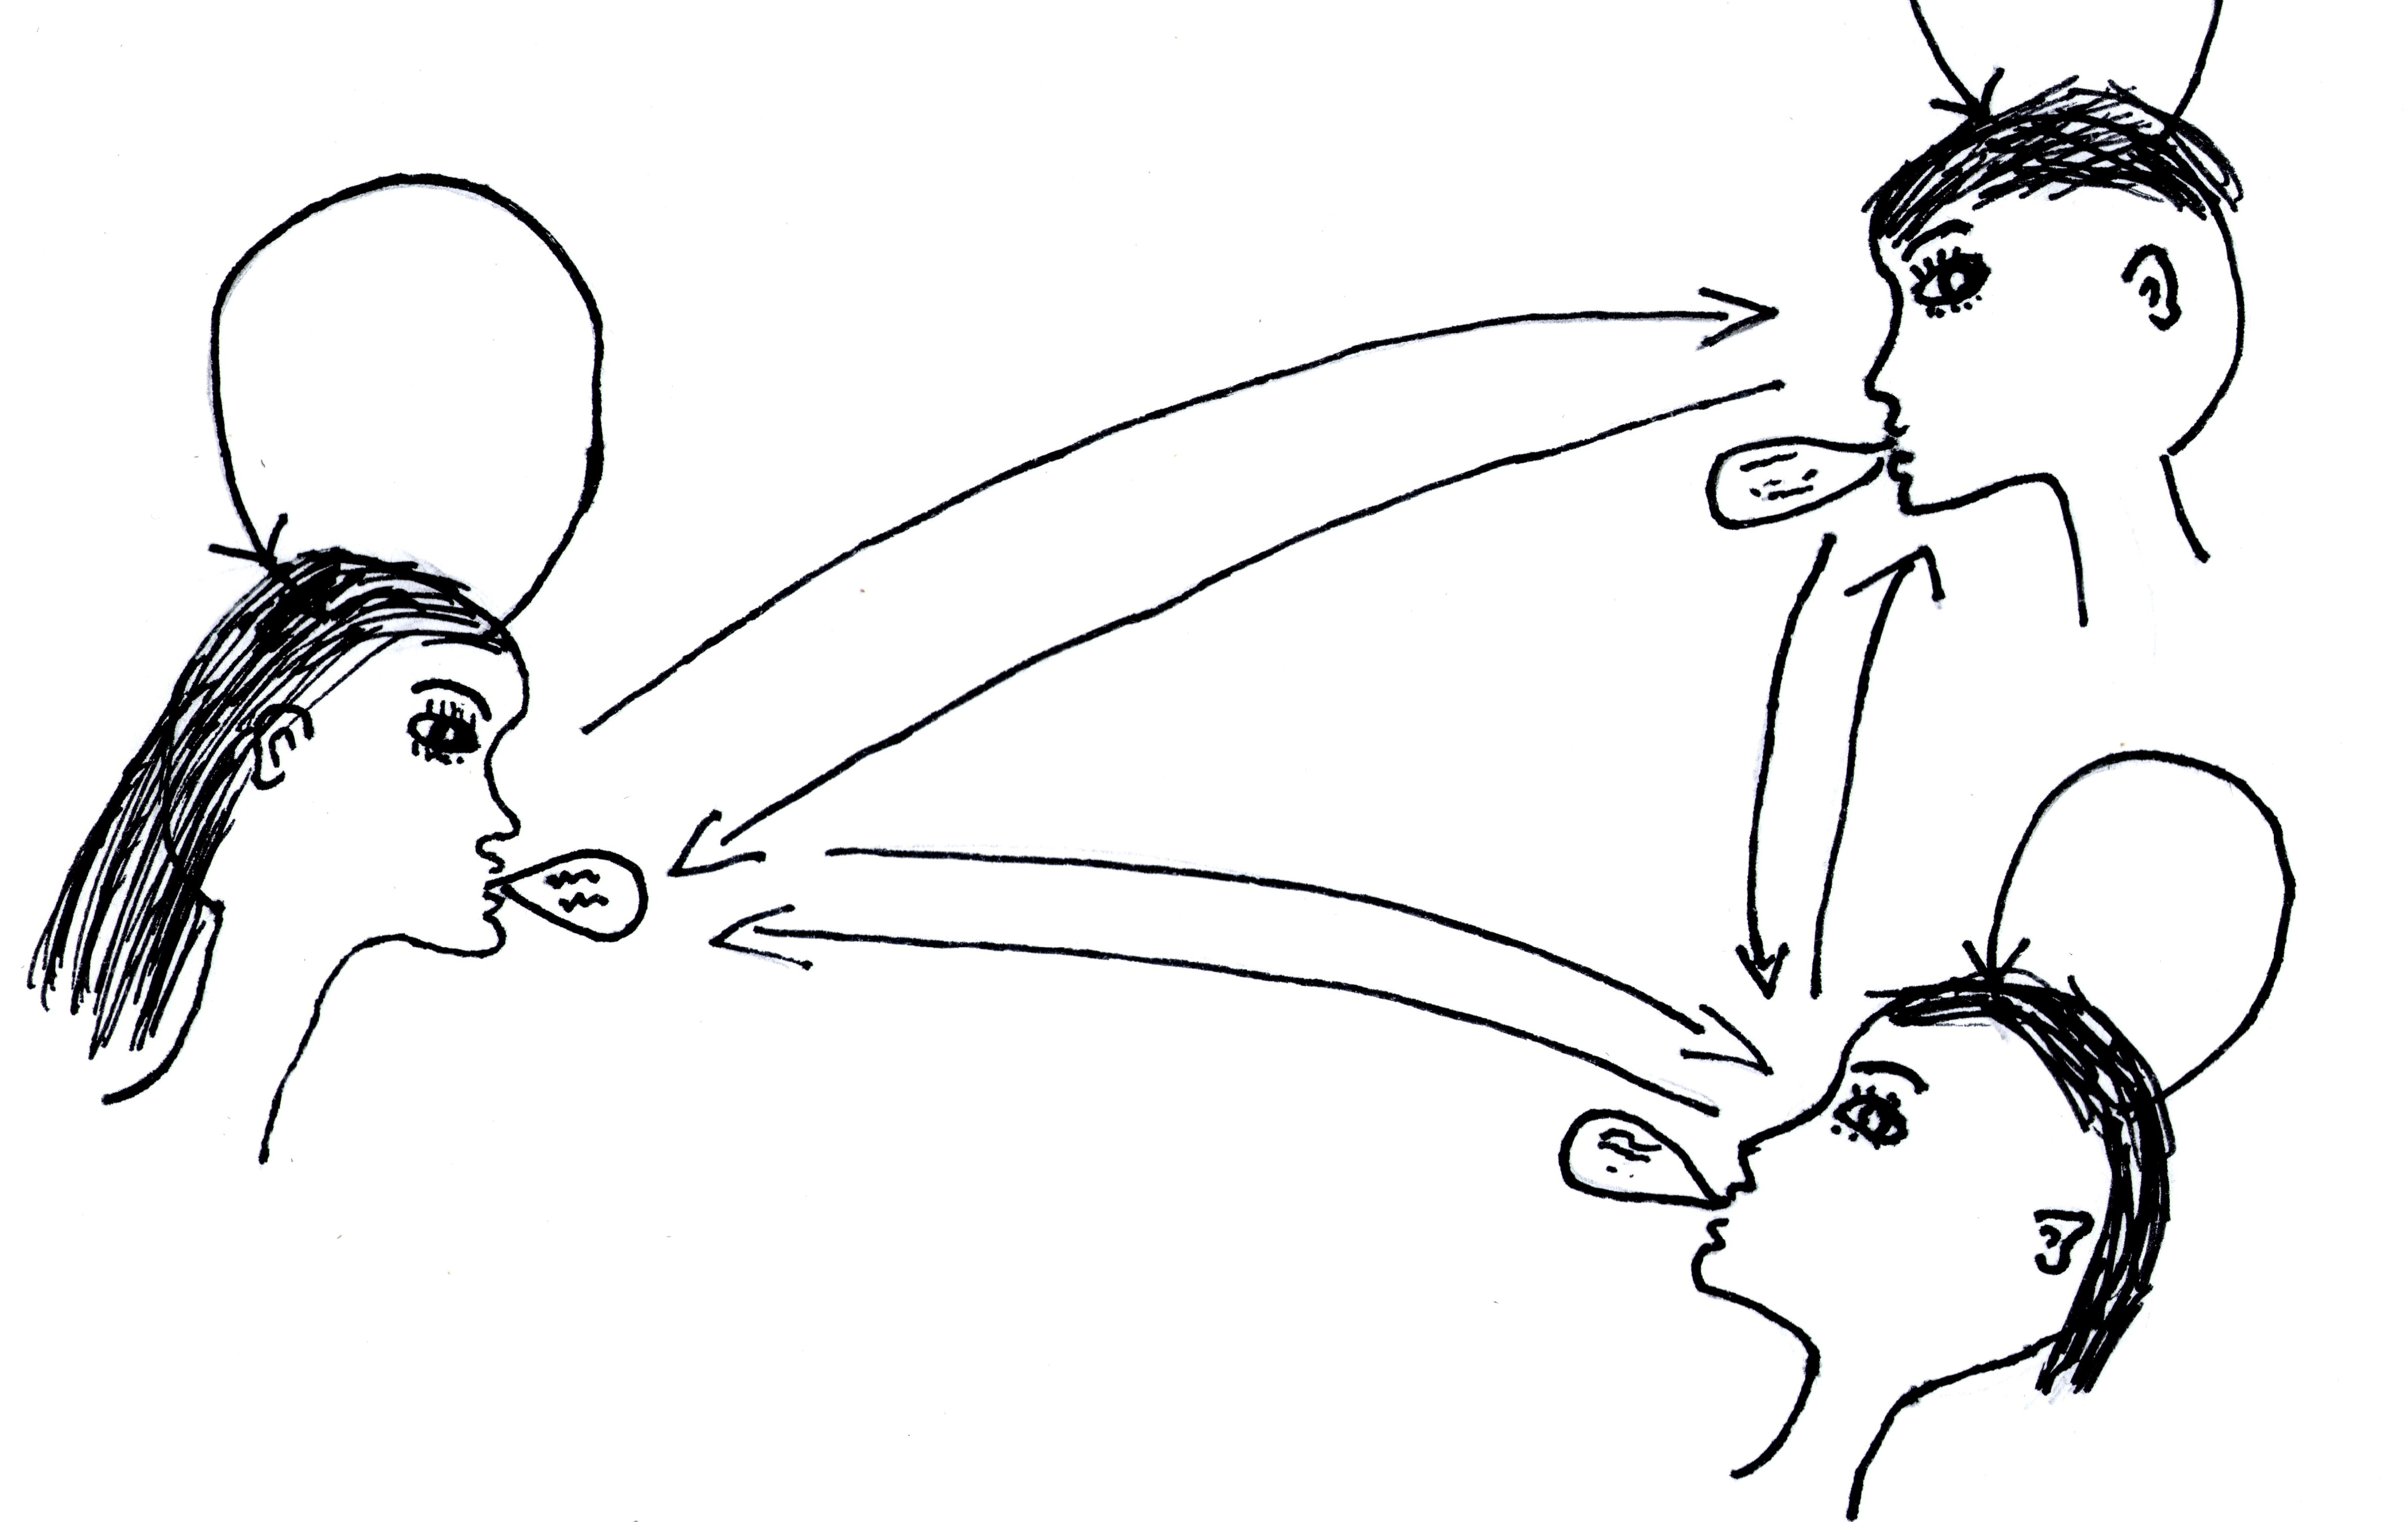
\includegraphics[width=0.6\textwidth]{grafiken/psycholinguistik/psycholinguistik.jpg}
\label{t9}
\end{center}
\end{figure}

\section{Stichworte zum Vortrag \em{Psycholinguistik}}

Mentales Lexikon, Spracherwerb, Sprachverarbeitung, Eye-Tracking-Methode, Lexical Decision

\newpage

\section{Übungen}



\subsection*{Fragestellungen}

Was könnten typische Fragestellungen in der Psycholinguistik sein? Welche Frage würden Sie gern untersuchen?

\vspace{4cm}

Diskutieren Sie, welche Ereignisse beobachtet und gemessen werden können. Was bedeutet das für psycholinguistische Experimente und deren Aussagen über mentale Prozesse?

\vspace{4cm}

\subsection*{Eyetracking}

Lesen Sie den Textausschnitt zum Eyetracking. Diskutieren Sie, welche Vorteile diese Methode hat und worauf beim Erstellen eines Experiments besonders geachtet werden muss.


\vspace{4cm}

\subsection*{Erstspracherwerb – Fremdspracherwerb}

Überlegen Sie in der Gruppe, was die Merkmale des Erst- und des Fremdspracherwerbs sind. Wie unterscheiden sich die beiden voneinander?

\vspace{4cm}

Überlegen Sie sich ein Beispiel und formulieren Sie eine wissenschaftliche Frage zum Fremdspracherwerb, die Sie gerne testen würden.

\vspace{4cm}

\newpage

\section{Literatur}
Aitchinson, J. (2012\super{4}). Words in the Mind: An Introduction to the Mental Lexicon. West Sussex: John Wiley \& Sons. \newline\\
Cutler, A.; Klein, W. \& Levinson, S. C. (2005). \textit{The cornerstones of twenty-first century psycholinguistics}. In: Twenty-first century psycholinguistics. Four cornerstones. Hg. von Anne Cutler.  Mahwah, New Jersey, London: Lawrence Erlbaum. 1–20.\newline\\
Dietrich, R. (2007). Psycholinguistik. Stuttgart, Weimar: J. B. Metzler.\newline\\
Göttert, K. H. (1991). Einführung in die Rhetorik. München: Wilhelm Fink Verlag.\newline\\
Huettig, F., Rommers, J., Meyer, A. S. (2001). Using the visual world paradigm to study language processing: A review and critical evaluation, Acta Psychologica, 137, Issue 2, 151-171\newline\\
Grimm, H. \& Weinert, S. (2002). \textit{Sprachentwicklung}. In: Oerter, R.; Montada, L. (Hrsg.): Entwicklungspsychologie (S. 517-550). Weinheim u.\,a.: Beltz.\newline\\
Herrmann, C.; Fiebach, C. (2004). Gehirn \& Sprache. Frankfurt am Main.\newline\\
Knobloch, Clemens (2003). \textit{Geschichte der Psycholinguistik}. In: Gerd R.; Herrmann, T. und Deutsch, W. (Hrsg.): Psycholinguistik. Psycholinguistics. Ein internationales Handbuch. An international handbook. Berlin, New York: Walter de Gruyter. 15–33.\newline\\
Koch, P. \& Oesterreicher, W. (1994). \textit{Schriftlichkeit und Sprache}. In: Günther, H.; Ludwig, O. (Hrsg.): Schrift und Schriftlichkeit. HSK. Berlin, New York: de Gruyter.\newline\\
Levelt, W. J. M.(1989). Speaking. From Intention to Articulation. Cambridge, MA; London: MIT Press.\newline\\
Osgood, C. E., und Thomas A. S. (Hrsg) (1954). \textit{Psycholinguistics. A survey of theory and research problems. Report of the 1953 summer seminar sponsored by the Committee on Linguistics and Psychology of the Social Science Research Council}. Baltimore: Waverly Press.\newline\\
Vygotskij, L. S. (1934/2002). Denken und Sprechen. Weinheim und Basel: Beltz.\newline\\
